% ============================================================
% Chapter 3 --- Open and closed sets
% Originally: content/week-02.tex, \section{Open and closed sets} plus the Friday
%             unit-ball warm-up (Corsin Week 2)
% ============================================================
\chapter{Open and Closed Sets}
\label{ch:open_closed}

% Transition: Claude Opus 5 (Medium)
With a distance in hand, the next question is which subsets a metric singles out. This chapter
introduces open balls, open and closed sets, and the interior, closure and boundary of a set, and
ends by looking at what the unit ball of each of the three standard metrics actually looks like
--- three visibly different shapes that nonetheless induce exactly the same open sets.

% Originally: content/week-02.tex, \section{Open and closed sets} (Corsin Week 2, Monday)

% Retitled from "Open and closed sets" now that the chapter carries that name; the label is
% unchanged, so every existing \cref still resolves.
\section{Open balls, open and closed sets}
\label{sec:open_closed_sets}

\begin{definition}[Open ball]
\label{def:open_ball}
Let $(X,d)$ be a metric space, let $x \in X$, and let $r \in \mathbb{R}$. Then we define the
\newterm{open ball} of radius $r$ as
\[B_r(x) := \{\,\boxed{y \in X}\, : d(y,x) < r\,\}\]
\end{definition}

\begin{importantremark}
Corsin marks the boxed part in red as an \qt{important subtlety}: the ambient set $X$ in
$y \in X$ is what makes openness relative to the space, and it is exactly what the common
misconception on \cref{rem:common_misconception} turns on.
\end{importantremark}

\begin{ainote}
\Cref{def:open_ball} is stated for $r \in \mathbb{R}$ rather than $r > 0$. Harmless here, but
loose.
\end{ainote}

% Moved here from before \cref{def:open_ball} (review item D1): it uses $B_r(x)$,
% "open" and "clopen", none of which were defined at its former position.
\begin{aiexample}[Open Balls in the Discrete Metric]
% Generator: Gemini 3.6 Flash (Medium)
Let $(X, d_{\text{disc}})$ be a discrete metric space. The open ball $B_r(x)$ centered at
$x \in X$ with radius $r > 0$ is
\[
B_r(x) = \begin{cases} \{x\} & \text{if } 0 < r \leq 1, \\ X & \text{if } r > 1. \end{cases}
\]
Hence every singleton $\{x\}$ is open in the discrete metric, and consequently every subset of
$X$ is both open and closed (\newterm{clopen}). This is exactly what \Cref{ex:X_empty_clopen}
below asks you to verify for $X$ and $\emptyset$ in a general metric space.
\end{aiexample}

% Generator: Claude Opus 5 (Medium)
\begin{remark}[Two degenerate balls worth knowing]
Taking \cref{def:open_ball} literally at the edges of its range is a cheap way to test whether
you have read it correctly.
\begin{itemize}
  \item If $r \leq 0$, then $B_r(x) = \emptyset$, and \emph{not} $\{x\}$. The condition is
    $d(y,x) < r$, strictly, and $d(x,x) = 0 \not< 0$. So even the centre is missing from
    $B_0(x)$.
  \item In the discrete metric $B_1(x) = \{x\}$, while $B_{1.01}(x) = X$: a ball can jump from a
    single point to the entire space without passing through anything in between. Radii do not
    have to behave like radii.
\end{itemize}
These are the two cases that make \qt{shrink the ball a little} arguments go wrong if applied
without thinking.
\end{remark}

% Generator: Claude Opus 5 (Medium)
\begin{aiexercise}[Open balls are open]
\label{ex:ai_open_balls_are_open}
The name promises it, but \cref{def:open_ball} does not say it. Show that in any metric space
$(X,d)$ the ball $B_r(x)$ is an open set in the sense of \cref{def:open_closed}.

\textit{Hint:} given $y \in B_r(x)$, the number $\varepsilon := r - d(y,x)$ is strictly positive.
Draw the picture, then let the triangle inequality do the work.
\end{aiexercise}

\begin{definition}[Open and closed sets]
\label{def:open_closed}
Then, we call a subset $U \subseteq X$ \newterm{open} (\germanterm{offen}) if and only if
\[\forall y \in U \ \exists \varepsilon > 0 \text{ such that } B_\varepsilon(y) \subseteq U.\]
And we call $A \subseteq X$ \newterm{closed} (\germanterm{abgeschlossen}) if and only if
$X \setminus A$ is open.
\end{definition}

\begin{center}
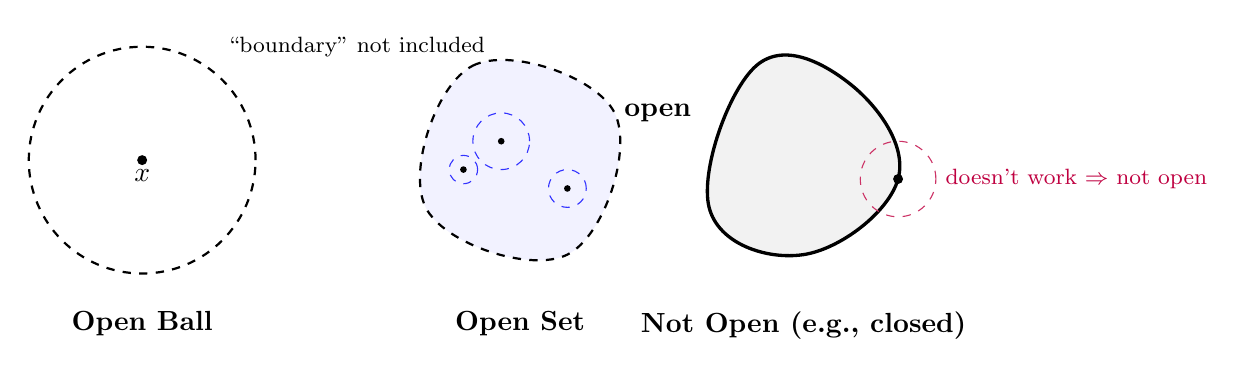
\begin{tikzpicture}[scale=1.2]
  % Open Ball
  \draw[dashed, thick] (0,0) circle (1.2);
  \fill (0,0) circle (1.5pt) node[below] {$x$};
  \node[anchor=west] at (0.8, 1.2) {\footnotesize ``boundary'' not included};
  \node[below] at (0, -1.5) {\textbf{Open Ball}};

  % Open set
  \begin{scope}[xshift=4cm]
    \draw[dashed, thick, fill=blue!5] 
      plot[smooth cycle, tension=0.7] coordinates {(-1,-0.5) (-0.5,1) (1,0.5) (0.5,-1)};
    \fill (-0.2,0.2) circle (1pt);
    \draw[dashed, blue!80] (-0.2,0.2) circle (0.3);
    \fill (0.5,-0.3) circle (1pt);
    \draw[dashed, blue!80] (0.5,-0.3) circle (0.2);
    \fill (-0.6,-0.1) circle (1pt);
    \draw[dashed, blue!80] (-0.6,-0.1) circle (0.15);
    \node[right, font=\bfseries] at (1, 0.5) {open};
    \node[below] at (0, -1.5) {\textbf{Open Set}};
  \end{scope}

  % Not Open set (Closed / boundary included)
  \begin{scope}[xshift=7cm]
    \draw[very thick, fill=gray!10] 
      plot[smooth cycle, tension=0.7] coordinates {(-1,-0.5) (-0.5,1) (0.5,0.8) (1,-0.2) (0,-1)};
    \fill (1,-0.2) circle (1.5pt);
    \draw[dashed, purple!80] (1,-0.2) circle (0.4);
    \node[purple, right] at (1.4, -0.2) {\footnotesize doesn't work $\Rightarrow$ not open};
    \node[below] at (0, -1.5) {\textbf{Not Open (e.g., closed)}};
  \end{scope}
\end{tikzpicture}
\end{center}

% Supplement: Analysis_II_Script_v1.pdf, p. 14
\begin{example}[Clopen sets other than $X$ and $\emptyset$]
\label{ex:clopen_nontrivial}
\Cref{ex:X_empty_clopen} shows $X$ and $\emptyset$ are always clopen, but nothing in
\cref{def:open_closed} forces these to be the \emph{only} clopen subsets of $X$. Take
$X := (0,1)\cup(2,3) \subset \mathbb{R}$ with the standard metric: both $(0,1)$ and $(2,3)$ are
clopen \emph{in $X$}. Each is open in $\mathbb{R}$, hence open in $X$; and each is the complement
in $X$ of the other, so each is also closed in $X$. Whether a space has clopen subsets besides
$X$ and $\emptyset$ turns out to be exactly the question \cref{ch:connectedness} is organised
around. A space with none is called \newterm{connected}.
\end{example}

% Supplement: Sascha Brack/Class Notes/Week_02_Notes_Friday_Updated.pdf, p. 1
\begin{proposition}[How open and closed sets combine]
\label{prop:open_closed_operations}
Let $(X,d)$ be a metric space.
\begin{enumerate}[label=\textbf{(\alph*)}]
  \item \label{item:arbitrary_union_open}
    \textbf{Arbitrary} unions of open sets are open: if $\{U_i\}_{i \in I}$ are open, so is
    $\bigcup_{i\in I}U_i$.
  \item \label{item:finite_intersection_open}
    \textbf{Finite} intersections of open sets are open: if $U_1,\dots,U_k$ are open, so is
    $\bigcap_{i=1}^{k}U_i$.
  \item \textbf{Arbitrary} intersections of closed sets are closed, and \textbf{finite} unions
    of closed sets are closed.
\end{enumerate}
\end{proposition}

\begin{proof}
\textbf{(a)} Let $x \in \bigcup_i U_i$. Then $x \in U_{i_0}$ for some $i_0$, and since $U_{i_0}$
is open there is $\varepsilon>0$ with $B_\varepsilon(x) \subseteq U_{i_0} \subseteq \bigcup_iU_i$.

\textbf{(b)} Let $x \in \bigcap_{i=1}^kU_i$. For each $i$ pick $\varepsilon_i>0$ with
$B_{\varepsilon_i}(x) \subseteq U_i$, and set $\varepsilon := \min\{\varepsilon_1,\dots,\varepsilon_k\}$.
Then $\varepsilon > 0$, and \emph{this is the only place finiteness is used}: a minimum of
finitely many positive numbers is positive, whereas an infimum of infinitely many can be $0$.
Since $B_\varepsilon(x) \subseteq U_i$ for every $i$, we conclude that
$B_\varepsilon(x) \subseteq \bigcap_iU_i$.

\textbf{(c)} Take complements and apply \textbf{(a)}, \textbf{(b)} via De Morgan:
$X\setminus\bigcap_iA_i = \bigcup_i(X\setminus A_i)$ and
$X\setminus\bigcup_{i=1}^kA_i = \bigcap_{i=1}^k(X\setminus A_i)$.
\end{proof}

% Generator: Claude Opus 5 (Medium)
\begin{importantremark}[The asymmetry is real, not an artefact of the proof]
\label{rem:finiteness_is_necessary}
It is tempting to read \qt{finite} in \textbf{(b)} as laziness. It is not: an infinite
intersection of open sets genuinely need not be open. In $\mathbb{R}$,
\[\bigcap_{n=1}^{\infty}\left(-\tfrac1n,\ \tfrac1n\right) = \{0\},\]
an intersection of open intervals which is not open. The proof shows exactly where it breaks:
$\varepsilon := \min_i\varepsilon_i$ is the whole argument, and an infimum of infinitely many
positive numbers can be $0$. Dually, $\bigcup_{n\geq1}\big[\tfrac1n,1\big] = (0,1]$ is an
infinite union of closed sets that is not closed.

\begin{ainote}
These four closure properties are exactly the axioms of a \newterm{topology}, which is how the
subject is set up when one drops the metric altogether (\cref{sec:structured_spaces},
\qt{fourth semester}). That is why they are worth isolating: they are the only facts about open
sets that survive into the general theory.
\end{ainote}
\end{importantremark}

% Supplement: Sascha Brack/Class Notes/Week_02_Notes_Friday_Updated.pdf, p. 1
\begin{example}[Open and closed sets in $\mathbb{R}$]
\label{ex:open_closed_R}
Consider the following subsets of $\mathbb{R}$ with the standard metric:
\begin{enumerate}[label=\textbf{(\alph*)}]
  \item \textbf{Is $\mathbb{N}$ open, closed, or neither?} It is \textbf{closed}, since its
    complement $\mathbb{R} \setminus \mathbb{N} = (-\infty, 1) \cup \bigcup_{n=1}^\infty (n, n+1)$
    is a union of open intervals, which is open by
    \Cref{prop:open_closed_operations}\textbf{\ref{item:arbitrary_union_open}}. It is not open,
    because no open ball around any $n \in \mathbb{N}$ is contained in $\mathbb{N}$.
  \item \textbf{Let $A := \{\frac{1}{n} \mid n = 1, 2, \dots\}$.} The set $A$ is \textbf{neither}
    open nor closed. It is not open for the same reason as $\mathbb{N}$. It is not closed because
    $0$ is an accumulation point of $A$, but $0 \notin A$, meaning its complement
    $\mathbb{R} \setminus A$ is not open (any open ball around $0$ intersects $A$).
  \item \textbf{Let $F := \{\frac{1}{n} \mid n = 1, 2, \dots\} \cup \{0\}$.} The set $F$ is
    \textbf{closed}. By adding the limit point $0$, the complement $\mathbb{R} \setminus F$
    becomes a union of open intervals, which is open.
\end{enumerate}
\end{example}

% Supplement: Linus Lüchinger/Slides/Slides-02-23.pdf, slide 20
% Linus's self-test list. The three entries Sascha already works above (N, {1/n},
% {1/n} u {0}) are dropped; what remains is the part that is not already answered.
\begin{exercise}[A longer self-test]
\label{ex:open_closed_self_test}
Linus sets the following list as a self-test at the end of his first session. Each subset of
$\mathbb{R}$ carries the standard metric; decide for each whether it is \textbf{open},
\textbf{closed}, \textbf{both}, or \textbf{neither}.
\begin{enumerate}[label=\textbf{(\alph*)}]
  \item $[0,\infty)$
  \item $\mathbb{Q}$
  \item $\{x - \lfloor x \rfloor : x \in \mathbb{R}\}$
  \item $S := \{x \in \mathbb{R} : x\cdot 2^p \in [1,2] \text{ for some integer } p \geq 0\}$
  \item $T := \{x \in \mathbb{R} : x\cdot 2^p \in (1,2) \text{ for some integer } p \geq 0\}$
  \item $\{x_n : n \in \mathbb{N}\}$, where $x_0 := 1$ and
    $x_n := \tfrac12\big(x_{n-1} + x_{n-1}^2\big)$
  \item $\{\Rea(c) : c \in \mathbb{C},\ \zeta(c) = 0\}$, where $\zeta$ is the Riemann zeta
    function
\end{enumerate}
Compare \textbf{(d)} with \textbf{(e)} before reading the solution: the two differ only in one
bracket.
\end{exercise}

% Quelle: Jérôme Paschoud/Notizen/Woche 2.1 Metrische Räume.pdf, p. 5
\begin{exercise}[Relative openness]
\label{ex:relative_openness_subsets}
Let $X := (\{0\} \times \mathbb{R}) \cup (0,1)^2$ be equipped with the subspace metric from $\mathbb{R}^2$. Consider the following subsets of $X$:
\begin{align*}
  A &:= \{(x,y) \in \mathbb{R}^2 \mid x = 0, y \in (2,3)\} \\
  B &:= \left\{(x,y) \in \mathbb{R}^2 \ \middle|\ \left(x - \tfrac12\right)^2 + \left(y - \tfrac12\right)^2 < \tfrac{1}{16}\right\}
\end{align*}
Are $A$ and $B$ open with respect to $X$? Are they open with respect to $\mathbb{R}^2$?
\end{exercise}

% Generator: Gemini 3.6 Pro
\begin{exercisesolution}[Proof of \cref{ex:relative_openness_subsets}]
\begin{itemize}
  \item $A$ is \textbf{open with respect to $X$}, but \textbf{not open with respect to $\mathbb{R}^2$}. It is open in $X$ because $A = X \cap U$ where $U = (-\varepsilon, \varepsilon) \times (2,3)$ is an open set in $\mathbb{R}^2$. It is not open in $\mathbb{R}^2$ because any open ball around a point in $A$ will contain points with $x \neq 0$, which are not in $A$.
  \item $B$ is \textbf{open with respect to both $X$ and $\mathbb{R}^2$}. $B$ is exactly the open ball $B_{1/4}((\tfrac12, \tfrac12))$ in $\mathbb{R}^2$, which is open in $\mathbb{R}^2$. Since $B \subseteq (0,1)^2 \subset X$, we have $B = X \cap B$, so $B$ is also open relative to $X$.
\end{itemize}
\end{exercisesolution}

% Originally: content/week-02.tex, the second half of \section{Open and closed sets}
% (Corsin Week 2, Monday) --- promoted to a section of its own, since the chapter
% otherwise consisted of one section carrying the chapter's own title.
\section{Interior, closure and boundary}
\label{sec:interior_closure_boundary}

% Sonnet 5 (Medium)
\begin{definition}[Interior, closure, and boundary]
\label{def:interior_closure_boundary}
Let $(X,d)$ be a metric space and $A \subseteq X$. The \newterm{interior}
(\germanterm{Inneres}) of $A$ is
\[\operatorname{int}(A) := \{x \in A : \exists\, r>0 \text{ such that } B_r(x) \subseteq A\},\]
the largest open subset of $X$ contained in $A$. The \newterm{closure} (\germanterm{Abschluss}) of
$A$ is
\[\overline{A} := \{x \in X : B_r(x) \cap A \neq \emptyset \text{ for all } r > 0\},\]
the smallest closed subset of $X$ containing $A$. The \newterm{boundary} (\germanterm{Rand}) of
$A$ is $\partial A := \overline{A} \setminus \operatorname{int}(A)$.
\end{definition}

\begin{aiexample}[Interior, Closure, and Boundary of an Interval]
% Generator: Gemini 3.6 Flash (Medium)
Applying \cref{def:interior_closure_boundary} to $A := (0,1] \subset \mathbb{R}$ under the
standard Euclidean metric:
\begin{itemize}
  \item The \textbf{interior} is $\operatorname{int}(A) = (0,1)$, the largest open set contained in $A$.
  \item The \textbf{closure} is $\overline{A} = [0,1]$, the smallest closed set containing $A$.
  \item The \textbf{boundary} is $\partial A = \overline{A} \setminus \operatorname{int}(A) = \{0, 1\}$.
\end{itemize}
Note that $1 \in A$ while $0 \notin A$: the boundary is not required to lie inside the set, nor
outside it. That is the point of defining it as a difference of two other sets rather than as
\qt{the edge of $A$}.
\end{aiexample}

% Generator: Claude Opus 5 (High) --- FIG-W02-01: the three notions in one picture.
\begin{center}
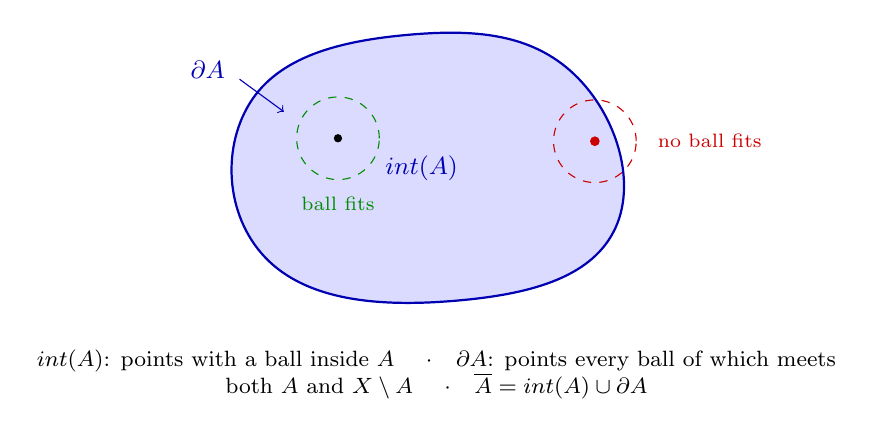
\begin{tikzpicture}[scale=1.25]
  % A blob A. int(A) is the shaded open part; the solid curve is dA; closure = both together.
  \draw[blue!70!black, thick, fill=blue!14, smooth cycle, tension=0.75]
    plot coordinates {(-1.7,-0.9) (-1.9,0.7) (-0.3,1.4) (1.4,1.0) (1.8,-0.6) (0.2,-1.3)};

  \node[blue!70!black, font=\small] at (-0.15,0.05) {$\operatorname{int}(A)$};

  % a point of the interior, with a ball that fits
  \fill (-1.0,0.35) circle (1.2pt);
  \draw[green!55!black, dashed] (-1.0,0.35) circle (0.42);
  \node[green!55!black, font=\scriptsize, below] at (-1.0,-0.15) {ball fits};

  % a boundary point: every ball meets A and its complement
  \fill[red!80!black] (1.61,0.32) circle (1.4pt);
  \draw[red!80!black, dashed] (1.61,0.32) circle (0.42);
  \node[red!80!black, font=\scriptsize, anchor=west] at (2.15,0.32) {no ball fits};

  \node[blue!70!black, font=\small, anchor=east] at (-2.05,1.05) {$\partial A$};
  \draw[blue!70!black, ->] (-2.0,0.95) -- (-1.55,0.62);

  \node[font=\footnotesize, align=center] at (0,-2.05)
    {$\operatorname{int}(A)$: points with a ball inside $A$ \quad$\cdot$\quad
     $\partial A$: points every ball of which meets\\
     both $A$ and $X\setminus A$ \quad$\cdot$\quad
     $\overline{A} = \operatorname{int}(A) \cup \partial A$};
\end{tikzpicture}
\end{center}

\begin{remark}[Interior and closure are dual]
\label{rem:interior_closure_dual}
The two constructions are not independent: taking complements swaps them,
\[X \setminus \operatorname{int}(A) = \overline{X\setminus A},
  \qquad\qquad
  X \setminus \overline{A} = \operatorname{int}(X\setminus A).\]
Both read off \cref{def:interior_closure_boundary} directly, since $x$ fails to have a ball inside
$A$ exactly when every ball around $x$ meets $X\setminus A$. In particular $\partial A =
\partial(X\setminus A)$: a set and its complement share their boundary, which is why the
boundary of the open disk and of its closed complement are the same circle.
\end{remark}

% Source: Corsin Nick/Class Notes/Week 2.pdf, p. 7
\begin{exercise}[$X$ and $\emptyset$ are clopen]
\label{ex:X_empty_clopen}
Let $(X,d)$ be a metric space. Show that $X$ and $\emptyset$ are both open and closed.
\end{exercise}

% Kept inline: solved directly in Corsin Nick/Class Notes/Week 2.pdf, p. 7.
\begin{exercisesolution}[Proof of \cref{ex:X_empty_clopen}]
$X$ is open, since $B_r(x) \subseteq X$ for all $r > 0$ and $x \in X$
(\cref{def:open_ball}). The empty set contains no
points and is therefore vacuously open. Since $X$ and $\emptyset$ are each other's complement in
$X$, they are also closed.
\end{exercisesolution}

% Supplement: Sascha Brack/Class Notes/Week_02_Notes_Friday_Updated.pdf, p. 2
\begin{example}[Interior, closure, and boundary in $\mathbb{R}$ and $\mathbb{R}^2$]
\label{ex:interior_closure_boundary_more}
Applying \cref{def:interior_closure_boundary} to various sets:
\begin{enumerate}[label=\textbf{(\alph*)}]
  \item Let $\Omega := \mathbb{Z} \subset \mathbb{R}$. Then $\operatorname{int}(\Omega) = \emptyset$ (no interval fits inside $\mathbb{Z}$), $\overline{\Omega} = \mathbb{Z}$ (it is already closed), and $\partial\Omega = \mathbb{Z} \setminus \emptyset = \mathbb{Z}$.
  \item Let $\Omega := B_1(0) \subset \mathbb{R}^2$. Then $\operatorname{int}(\Omega) = B_1(0)$ (it is already open), the closure is the closed disk $\overline{\Omega} = \{x \in \mathbb{R}^2 \mid d(x,0) \leq 1\}$, and the boundary is the unit circle $\partial\Omega = \{x \in \mathbb{R}^2 \mid d(x,0) = 1\}$.
  \item Let $\Omega := \mathbb{Q} \subset \mathbb{R}$. Then $\operatorname{int}(\Omega) = \emptyset$ (every open interval contains irrationals), $\overline{\Omega} = \mathbb{R}$ (every open interval contains rationals, so every real number is a closure point), and $\partial\Omega = \mathbb{R} \setminus \emptyset = \mathbb{R}$.
\end{enumerate}
\end{example}

% Supplement: Analysis_II_Script_v1.pdf, p. 15
\begin{exercise}[Closure and boundary of a ball in $\mathbb{R}^n$]
\label{ex:closure_boundary_of_ball}
For balls $B_r(x)$ in $\mathbb{R}^n$ with the Euclidean metric, prove that
\[\overline{B_r(x)} = \{y \in \mathbb{R}^n : d(x,y) \leq r\}\]
and deduce $\partial B_r(x) = \{y \in \mathbb{R}^n : d(x,y) = r\}$.
\end{exercise}

\begin{remark}
Item \textbf{(b)} of \cref{ex:interior_closure_boundary_more} above is exactly the case $r=1$,
$x=0$, $n=2$ of this exercise, worked here for general $x$, $r$ and $n$.
\end{remark}

% Quelle: Jérôme Paschoud/Notizen/Woche 2.1 Metrische Räume.pdf, p. 6
\begin{exercise}[Interior, closure, and boundary of a mixed set]
\label{ex:interior_closure_boundary_mixed}
Let $E := (\{0\} \times \mathbb{R}) \cup (0,1)^2 \subset \mathbb{R}^2$. Find the interior $\operatorname{int}(E)$, the closure $\overline{E}$, and the boundary $\partial E$ with respect to the standard metric on $\mathbb{R}^2$.
\end{exercise}

% Generator: Gemini 3.6 Pro
\begin{exercisesolution}[Proof of \cref{ex:interior_closure_boundary_mixed}]
\begin{itemize}
  \item \textbf{Interior:} $\operatorname{int}(E) = (0,1)^2$. The line $\{0\} \times \mathbb{R}$ contains no 2D open balls, so it contributes nothing to the interior. The open square $(0,1)^2$ is already open in $\mathbb{R}^2$.
  \item \textbf{Closure:} $\overline{E} = (\{0\} \times \mathbb{R}) \cup [0,1]^2$. The line $\{0\} \times \mathbb{R}$ is closed. The closure of the open square is the closed square $[0,1]^2$. The closure of a finite union is the union of the closures.
  \item \textbf{Boundary:} $\partial E = \overline{E} \setminus \operatorname{int}(E) = (\{0\} \times \mathbb{R}) \cup \big([0,1]^2 \setminus (0,1)^2\big)$. The second term is the perimeter of the square.
\end{itemize}
\end{exercisesolution}

% Originally: content/week-02.tex, the Friday warm-up following \subsection{Sequences and convergence}
% Corsin used this to reopen the topic on the Friday; it needs \cref{def:open_ball}, so it is
% placed here, after the open/closed material, rather than where the week happened to put it.
\section{Unit balls of the three standard metrics}
\label{sec:unit_balls}

\begin{warmup}
What is the shape of $B_1(0) \subseteq \mathbb{R}^2$ with the supremum metric? With the Manhattan
metric?
\end{warmup}

\begin{answer}
Supremum: the axis-aligned \textbf{open square} $(-1,1)^2$. Manhattan: the \textbf{open diamond}
$\{|x_1|+|x_2| < 1\}$. In both cases the strict inequality in \cref{def:open_ball} matters: the
points $(\pm 1,0)$ and $(0,\pm 1)$ sit on the boundary and are \emph{not} in the ball. They are
the corners of the diamond and the edge midpoints of the square, and are drawn hollow below.
\end{answer}


\begin{center}
\begin{tikzpicture}[>=Latex, scale=1.2]
  \begin{scope}[shift={(0,0)}]
    \draw[->] (-1.5,0) -- (1.5,0) node[right] {$x_1$};
    \draw[->] (0,-1.5) -- (0,1.5) node[above] {$x_2$};
    \draw[blue!80!black, thick, dashed, fill=blue!10] (-1,-1) rectangle (1,1);
    % Hollow: (1,0) and (0,1) have d_3 = 1, so they are NOT in the open ball B_1(0).
    \draw[orange!90!black, thick, fill=white] (1,0) circle (2pt);
    \node[orange!90!black, above right, font=\footnotesize] at (1,0) {$(1,0)$};
    \draw[orange!90!black, thick, fill=white] (0,1) circle (2pt);
    \node[orange!90!black, above right, font=\footnotesize] at (0,1) {$(0,1)$};
    \node[below, font=\small, align=center] at (0,-1.6)
      {Supremum metric $d_3$:\\ open square $(-1,1)^2$};
  \end{scope}

  \begin{scope}[shift={(4.4,0)}]
    \draw[->] (-1.5,0) -- (1.5,0) node[right] {$x_1$};
    \draw[->] (0,-1.5) -- (0,1.5) node[above] {$x_2$};
    \draw[blue!80!black, thick, dashed, fill=blue!10] (1,0) -- (0,1) -- (-1,0) -- (0,-1) -- cycle;
    % Same here: d_1((1,0),0) = 1, so the corners are boundary points, not elements.
    \draw[orange!90!black, thick, fill=white] (1,0) circle (2pt);
    \node[orange!90!black, above right, font=\footnotesize] at (1,0) {$(1,0)$};
    \draw[orange!90!black, thick, fill=white] (0,1) circle (2pt);
    \node[orange!90!black, above right, font=\footnotesize] at (0,1) {$(0,1)$};
    \node[below, font=\small, align=center] at (0,-1.6)
      {Manhattan metric $d_1$:\\ open diamond};
  \end{scope}

  \begin{scope}[shift={(8.8,0)}]
    \draw[->] (-1.5,0) -- (1.5,0) node[right] {$x_1$};
    \draw[->] (0,-1.5) -- (0,1.5) node[above] {$x_2$};
    \draw[blue!80!black, thick, dashed, fill=blue!10] (0,0) circle (1);
    \draw[orange!90!black, thick, fill=white] (1,0) circle (2pt);
    \node[orange!90!black, above right, font=\footnotesize] at (1,0) {$(1,0)$};
    \draw[orange!90!black, thick, fill=white] (0,1) circle (2pt);
    \node[orange!90!black, above right, font=\footnotesize] at (0,1) {$(0,1)$};
    \node[below, font=\small, align=center] at (0,-1.6)
      {Standard metric $d_2$:\\ open disk};
  \end{scope}
\end{tikzpicture}
\end{center}

% Generator: Claude Opus 5 (High)
\begin{remark}[The unit ball remembers which metric it came from]
\label{rem:unit_balls_distinguish_metrics}
Three metrics, three unmistakably different unit balls: the square for $d_3$, the disk for
$d_2$, the diamond for $d_1$. This is the quickest way to tell the three apart, and it also makes
\cref{ex:ai_metric_equivalence} visible, since the inclusions
\[B^{d_1}_1(0) \ \subseteq\ B^{d_2}_1(0) \ \subseteq\ B^{d_3}_1(0)\]
are precisely the inequalities $d_3 \leq d_2 \leq d_1$ read backwards. The larger the metric, the
harder it is to be within distance $1$, and hence the smaller the ball. The same family, continued
to all $p \geq 1$, is sketched in \cref{ex:4.3}\textbf{.1}, where the square reappears as the
limiting case $p \to \infty$.

None of this changes which sets are open. All three metrics have the same open sets, as
\cref{ex:ai_metric_equivalence} shows. The balls look different, and the topology does not notice.
\end{remark}



% Originally: content/week-02.tex, end of \section{Compactness}

\begin{aiexercise}[Boundary of the Open Unit Disk]
\label{ex:ai_disk_boundary}
% Generator: Gemini 3.6 Flash (Medium)
Let $D := \{(x,y) \in \mathbb{R}^2 \mid x^2 + y^2 < 1\}$ be the open unit disk in $\mathbb{R}^2$. Show that the boundary of $D$ is the unit circle $\partial D = \{(x,y) \in \mathbb{R}^2 \mid x^2 + y^2 = 1\}$.
\end{aiexercise}



% --- exercises relocated here from the dissolved sheet 2 ---

% Originally: content/exercise-sheets/week-02.tex, problem 2.2
% Source: exercises/Ex2_Analysis2_eng.pdf, p. 1

\begin{exercise}[2.2 --- Multiple choice (closure)]
\label{ex:2.2}
Let $(X,d)$ be a metric space, and $Y_1, Y_2 \subset X$ subsets. Select all the statements below
that are necessarily true.
\begin{enumerate}[label=\textbf{(\alph*)}]
  \item $\overline{Y_1 \cup Y_2} = \overline{Y_1} \cup \overline{Y_2}$
  \item $\overline{Y_1} \cap \overline{Y_2} \subset \overline{Y_1 \cap Y_2}$
  \item $\overline{Y_1 \cap Y_2} \subset \overline{Y_1} \cap \overline{Y_2}$
  \item $\overline{Y_1 \cap Y_2} = \overline{Y_1} \cap \overline{Y_2}$
\end{enumerate}
\exhint[Official hints]{\textbf{(b):} compare with \cref{ex:2.1}.3. \textbf{(d):} play with a set
of three points (a triangle).}
\end{exercise}

% Originally: content/exercise-sheets/week-02.tex, problem 2.3
% Source: exercises/Ex2_Analysis2_eng.pdf, p. 1

\begin{exercise}[2.3 --- Multiple choice (distance from a set)]
\label{ex:2.3}
Let $(X,d)$ be a metric space, and $A \subset X$ a non-empty subset. We define the function
``distance from $A$'' as
\[
  d(\cdot, A) : X \to [0,\infty), \qquad d(x,A) := \inf_{a \in A} d(x,a).
\]
Select all the statements below that are necessarily true.
\begin{enumerate}[label=\textbf{(\alph*)}]
  \item If $A$ is closed and $x \in A^c$, then $d(x,A) > 0$.
  \item The set $M := \{x \in X : d(x,A) \geq 1\}$ is closed in $X$.
  \item For $x, y \in X$, $d(x,A) \leq d(x,y) + d(y,A)$ holds.
  \item If $A^\circ$ is non-empty and $x \in X$, then $d(x,A) = d(x, A^\circ)$.
\end{enumerate}
\exhint[Official hint]{First convince yourself with a drawing that the name of this function is
appropriate; then use the characterization of open/closed sets with sequences.}
\end{exercise}

% Originally: content/exercise-sheets/week-02.tex, problem 2.4
% Source: exercises/Ex2_Analysis2_eng.pdf, p. 1

\begin{exercise}[2.4 --- Boundary, Interior etc.]
\label{ex:2.4}
Determine the interior, closure, and boundary of the following subsets $Y$ of $\mathbb{R}$, for
the standard topology on $\mathbb{R}$. No need to justify the answer.
\begin{center}
\begin{tabular}{ll ll}
(1) & $Y = [0,1]$ & (2) & $Y = \mathbb{Q}$ \\
(3) & $Y = \emptyset$ & (4) & $Y = (0,1)$ \\
(5) & $Y = [-1,1) \setminus \{0\}$ & (6) & $Y = [0,\infty)$ \\
(7) & $Y = \{0\}$ & (8) & $Y = \left\{\tfrac{1}{n} \mid n \in \mathbb{N}\setminus\{0\}\right\}$
\end{tabular}
\end{center}
\end{exercise}

% Originally: the \section{Solutions} of content/week-02.tex

\section{Solutions}
\label{sec:open_closed_solutions}

\begin{exercisesolution}[Proof of \cref{ex:ai_open_balls_are_open}]
% Generator: Claude Opus 5 (Medium)
Let $y \in B_r(x)$, so $d(y,x) < r$, and set $\varepsilon := r - d(y,x) > 0$. We claim that
$B_\varepsilon(y) \subseteq B_r(x)$, which is exactly what \cref{def:open_closed} requires.

Let $z \in B_\varepsilon(y)$, so $d(z,y) < \varepsilon$. By the triangle inequality
(\cref{def:metric_space}),
\[d(z,x) \leq d(z,y) + d(y,x) < \varepsilon + d(y,x) = \big(r-d(y,x)\big) + d(y,x) = r,\]
so $z \in B_r(x)$. Since $y \in B_r(x)$ was arbitrary, $B_r(x)$ is open.

\begin{remark}
The entire content is the choice $\varepsilon := r - d(y,x)$: the radius left over after
travelling from the centre out to $y$. Note that it shrinks to $0$ as $y$ approaches the edge of
the ball, so no \emph{single} $\varepsilon$ works for every $y$ at once. That is the same
\qt{the constant depends on the point} phenomenon which separates continuity from uniform
continuity in \cref{rem:continuity_vs_uniform_continuity}, met here for the first time.
\end{remark}
\end{exercisesolution}

\begin{exercisesolution}[Proof of \cref{ex:ai_disk_boundary}]
% Generator: Gemini 3.6 Flash (Medium)
Since $D$ is open, its interior is $\operatorname{int}(D) = D$. The closure of $D$ is $\overline{D} = \{(x,y) \in \mathbb{R}^2 \mid x^2 + y^2 \leq 1\}$. By \cref{def:interior_closure_boundary}, the boundary is:
\begin{align*}
\partial D &= \overline{D} \setminus \operatorname{int}(D) \\
&= \{(x,y) \in \mathbb{R}^2 \mid x^2 + y^2 \leq 1\} \setminus \{(x,y) \in \mathbb{R}^2 \mid x^2 + y^2 < 1\} \\
&= \{(x,y) \in \mathbb{R}^2 \mid x^2 + y^2 = 1\}.
\end{align*}
\end{exercisesolution}

% ===========================================================================
% Official sheet 2 (2.1--2.7). Derived independently, then checked against
% exercises/Sol2_Analysis2_eng.pdf.
% ===========================================================================

\begin{exercisesolution}[Solution to \cref{ex:2.2}]
% Generator: Claude Opus 5 (High)
\textbf{(a) and (c) are necessarily true; (b) and (d) are not.}

\textbf{(a) True.} Both inclusions come from general properties of the closure. Since
$Y_i \subseteq Y_1 \cup Y_2$ and the closure is monotone,
$\overline{Y_i} \subseteq \overline{Y_1\cup Y_2}$ for $i=1,2$, which gives \qt{$\supseteq$}.
Conversely $\overline{Y_1}\cup\overline{Y_2}$ is a \emph{finite} union of closed sets, hence
closed (\cref{prop:open_closed_operations}\textbf{(c)}), and it contains $Y_1\cup Y_2$; since
$\overline{Y_1\cup Y_2}$ is the smallest closed set containing $Y_1 \cup Y_2$
(\cref{def:interior_closure_boundary}), \qt{$\subseteq$} follows.

\textbf{(c) True,} and it is the easy half: $Y_1\cap Y_2 \subseteq Y_i$ gives
$\overline{Y_1\cap Y_2} \subseteq \overline{Y_i}$ for each $i$ by monotonicity, hence
$\overline{Y_1\cap Y_2} \subseteq \overline{Y_1}\cap\overline{Y_2}$.

\textbf{(b) False,} and therefore \textbf{(d) False} as well, (d) being (b) and (c) combined. In
$\mathbb{R}$ take
\[Y_1 := (0,1), \qquad Y_2 := (1,2).\]
Then $\overline{Y_1}\cap\overline{Y_2} = [0,1]\cap[1,2] = \{1\}$, whereas
$Y_1\cap Y_2 = \emptyset$ and so $\overline{Y_1\cap Y_2} = \emptyset$. The two sets meet only in
the limit, and the closure of the intersection cannot see a point belonging to neither set.

\begin{remark}[Where finiteness enters, again]
Part \textbf{(a)} is false for infinite unions, for exactly the reason given in
\cref{rem:finiteness_is_necessary}. Taking $Y_q := \{q\}$ for each $q \in \mathbb{Q}$,
\[\bigcup_{q\in\mathbb{Q}}\overline{Y_q} = \mathbb{Q}
  \qquad\text{but}\qquad
  \overline{\bigcup_{q\in\mathbb{Q}}Y_q} = \overline{\mathbb{Q}} = \mathbb{R}.\]
So the honest statement is: the closure commutes with \emph{finite} unions, and only
one-directionally with intersections. That is the same asymmetry that runs through the whole of
\cref{prop:open_closed_operations}.
\end{remark}
\end{exercisesolution}

\begin{exercisesolution}[Solution to \cref{ex:2.3}]
% Generator: Claude Opus 5 (High)
\textbf{(a), (b) and (c) are necessarily true; (d) is not.} It is efficient to prove
\textbf{(c)} first, since \textbf{(b)} then follows from it.

\textbf{(c) True.} Fix $x,y \in X$. For every $a \in A$ the triangle inequality gives
$d(x,a) \leq d(x,y) + d(y,a)$, and the left-hand side is bounded below by $d(x,A)$, so
\[d(x,A) \leq d(x,y) + d(y,a) \qquad\text{for every } a \in A.\]
Taking the infimum over $a$ on the right yields $d(x,A) \leq d(x,y) + d(y,A)$. Exchanging $x$
and $y$ and combining,
\[\big|d(x,A) - d(y,A)\big| \leq d(x,y),\]
so $d(\cdot,A)$ is \textbf{$1$-Lipschitz} (\cref{def:lipschitz_continuous}), in particular
continuous --- which is what the remaining parts use.

\textbf{(a) True.} If $A$ is closed then $A^c$ is open, so for $x \in A^c$ there is $r>0$ with
$B_r(x) \subseteq A^c$. No point of $A$ lies in that ball, i.e.\ $d(x,a) \geq r$ for every
$a \in A$, and taking the infimum gives $d(x,A) \geq r > 0$.

\textbf{(b) True.} By \textbf{(c)} the function $d(\cdot,A)$ is continuous, and
$M = d(\cdot,A)^{-1}\big([1,\infty)\big)$ is the preimage of a closed set under a continuous
map, hence closed (\cref{def:continuous}\textbf{(c)}, applied to complements).

\textbf{(d) False.} In $\mathbb{R}$ take $A := [0,1]\cup\{2\}$, whose interior
$A^\circ = (0,1)$ is non-empty as required. At the point $x := 2$,
\[d(x,A) = 0 \quad\text{(because } 2 \in A\text{)}, \qquad\qquad
  d(x,A^\circ) = \inf_{a\in(0,1)}|2-a| = 1.\]
The isolated point $2$ of $A$ contributes to $d(\cdot,A)$ but is invisible to $A^\circ$. The
hypothesis \qt{$A^\circ$ is non-empty} is far too weak, because it constrains $A$ nowhere near
$x$; the statement would become true under a hypothesis such as $A = \overline{A^\circ}$.
\end{exercisesolution}

\begin{exercisesolution}[Solution to \cref{ex:2.4}]
% Generator: Claude Opus 5 (High)
All with respect to the standard metric on $\mathbb{R}$, using
\cref{def:interior_closure_boundary}.
\begin{center}
\begin{tabular}{@{}c l l l l@{}}
& \textbf{$Y$} & \textbf{$\operatorname{int}(Y)$} & \textbf{$\overline{Y}$} & \textbf{$\partial Y$} \\
\hline
(1) & $[0,1]$ & $(0,1)$ & $[0,1]$ & $\{0,1\}$ \\
(2) & $\mathbb{Q}$ & $\emptyset$ & $\mathbb{R}$ & $\mathbb{R}$ \\
(3) & $\emptyset$ & $\emptyset$ & $\emptyset$ & $\emptyset$ \\
(4) & $(0,1)$ & $(0,1)$ & $[0,1]$ & $\{0,1\}$ \\
(5) & $[-1,1)\setminus\{0\}$ & $(-1,0)\cup(0,1)$ & $[-1,1]$ & $\{-1,0,1\}$ \\
(6) & $[0,\infty)$ & $(0,\infty)$ & $[0,\infty)$ & $\{0\}$ \\
(7) & $\{0\}$ & $\emptyset$ & $\{0\}$ & $\{0\}$ \\
(8) & $\left\{\tfrac1n : n \geq 1\right\}$ & $\emptyset$ &
  $\left\{\tfrac1n : n \geq 1\right\}\cup\{0\}$ &
  $\left\{\tfrac1n : n \geq 1\right\}\cup\{0\}$ \\
\end{tabular}
\end{center}

Three rows repay a second look.
\begin{itemize}
  \item \textbf{(1) versus (4).} The closed interval and the open interval have the same
    interior, the same closure and the same boundary. These three operations simply cannot
    distinguish a set from any other set squeezed between its interior and its closure.
  \item \textbf{(5).} Removing the single point $0$ from $[-1,1)$ adds $0$ to the boundary
    without changing the closure: a removed interior point becomes a boundary point. Note also
    that $1 \in \partial Y$ although $1 \notin Y$, while $-1 \in \partial Y$ and $-1 \in Y$ ---
    the boundary is indifferent to membership.
  \item \textbf{(2) and (8).} Both have empty interior, so $\partial Y = \overline{Y}$: once a
    set has no interior, the boundary swallows the entire closure. That is the general reason
    for $\partial\mathbb{Q} = \mathbb{R}$ in
    \cref{ex:interior_closure_boundary_more}\textbf{(c)}, and not an accident of $\mathbb{Q}$.
\end{itemize}
\end{exercisesolution}

